
\documentclass[12pt,a4paper]{scrartcl}		% KOMA-Klassen benutzen!

\usepackage[utf8]{inputenc}			% Zeichensatzkodierung
\usepackage{graphicx}				% Einbinden von Bildern
\usepackage{color}				% Farben wenn es sein muß
\usepackage{amsmath}		
\usepackage{amsfonts}
\usepackage{listings}

\definecolor{codegreen}{rgb}{0,0.6,0}
\definecolor{codegray}{rgb}{0.5,0.5,0.5}
\definecolor{codepurple}{rgb}{0.58,0,0.82}
\definecolor{backcolour}{rgb}{0.95,0.95,0.95}

\lstdefinestyle{mystyle}{
    backgroundcolor=\color{backcolour},   
    commentstyle=\color{codegreen},
    keywordstyle=\color{magenta},
    numberstyle=\tiny\color{codegray},
    stringstyle=\color{codepurple},
    basicstyle=\ttfamily\footnotesize,
    breakatwhitespace=false,         
    breaklines=true,                 
    captionpos=b,                    
    keepspaces=true,                 
    numbers=left,                    
    numbersep=5pt,                  
    showspaces=false,                
    showstringspaces=false,
    showtabs=false,                  
    tabsize=2
}

\lstset{style=mystyle}

\newcommand\svthema{INF264 Project 1}
\newcommand\svperson{Sophie Blum and Benjamin Friedl}
\newcommand\svdatum{18.09.2020}
\newcommand\lvname{Implementing decision trees}
\begin{document}

\title{ \svthema}
\author{\textsc{\lvname}}
\date{ \small \textsl{\svperson} --- \svdatum }
\maketitle

\abstract
About the document:
The names behind every title point out, who initially wrote the code for this functionality. 
The largest amount of time however went into debugging and correcting the code, as well as re-evaluating the 
design choices and making the algorithm work. We did all this together, so that it is hard to point out, who 
did what exactly.

\section{Preprocessing(Sophie)}
\subsection{Visualization}
To get a first idea of the distribution of the datapoints, we visualize them all together in the same graph (figure \ref{fig::all})
This graph gives a first idea of the curvature of the graph, but there are too many datapoints to see patterns directly.
\begin{figure}[h]
    \centering
    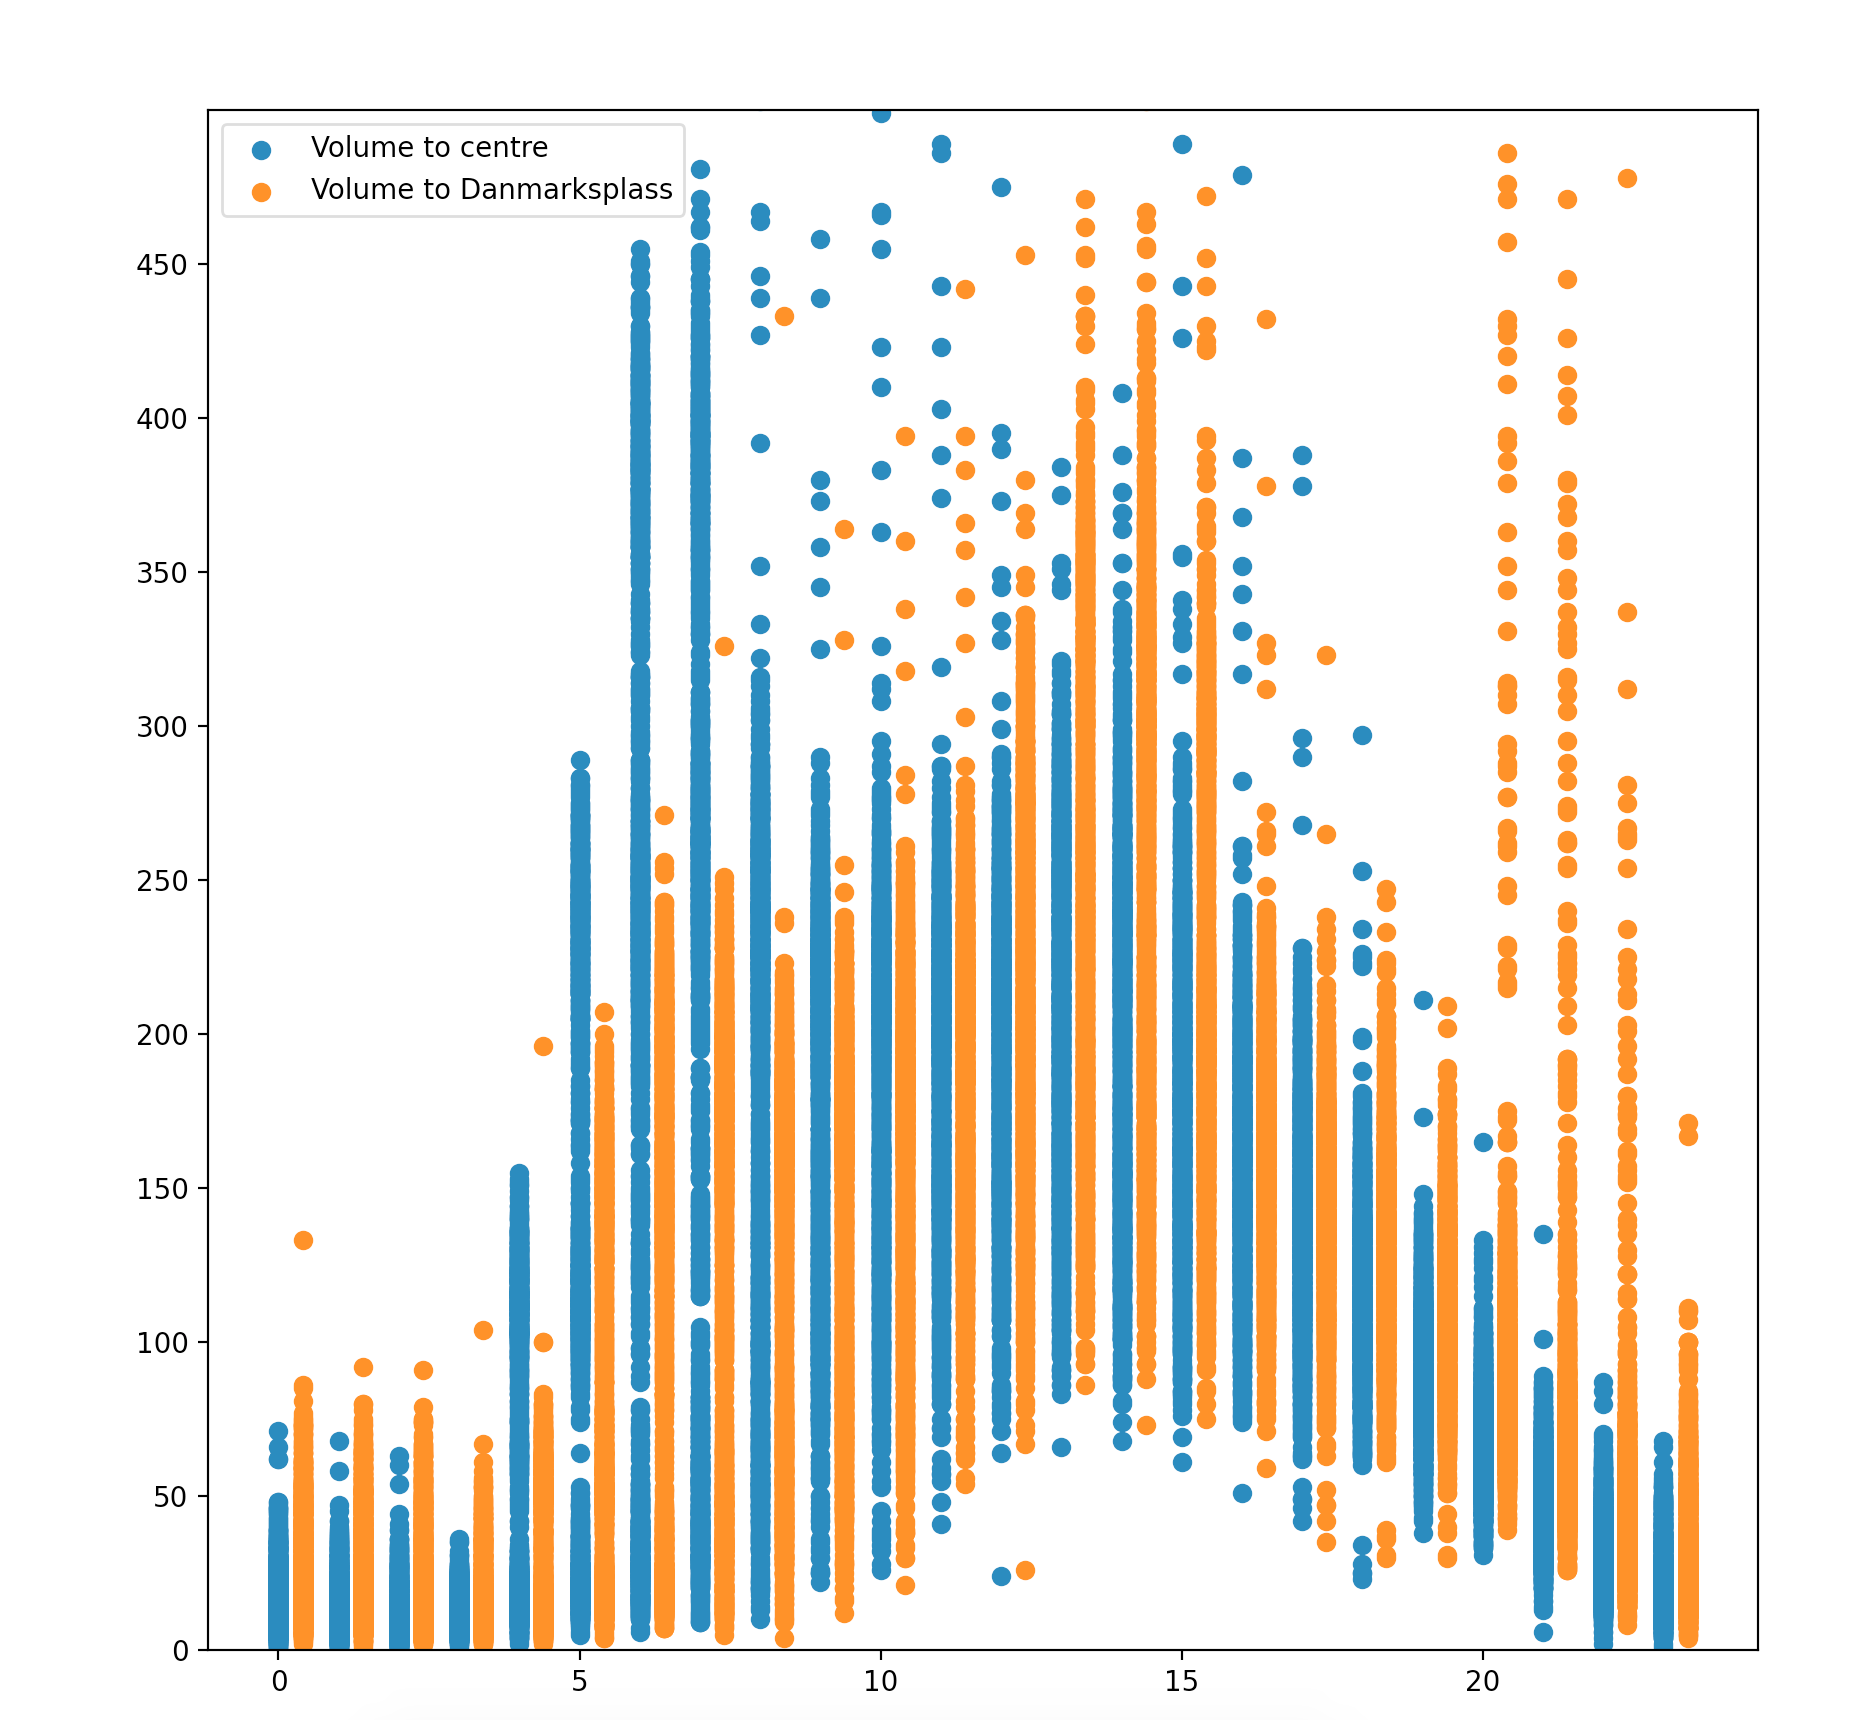
\includegraphics[scale = 0.45]{vis_all.png}
    \caption{All datapoints in one graph}
    \label{fig::all}
\end{figure}

We assume that the traffic volume varies for every weekday or at least from weekdays to sundays. To confirm our assumption, we seperate 
the datapoints according to their weekdays. To achieve that we use datetime objects for each datapoint and the \texttt{weekday()} function.
We also visualize the two directions in seperate colours to compare them in the same diagram (figure \ref{fig::days}).
\begin{figure}[h]
    \centering
    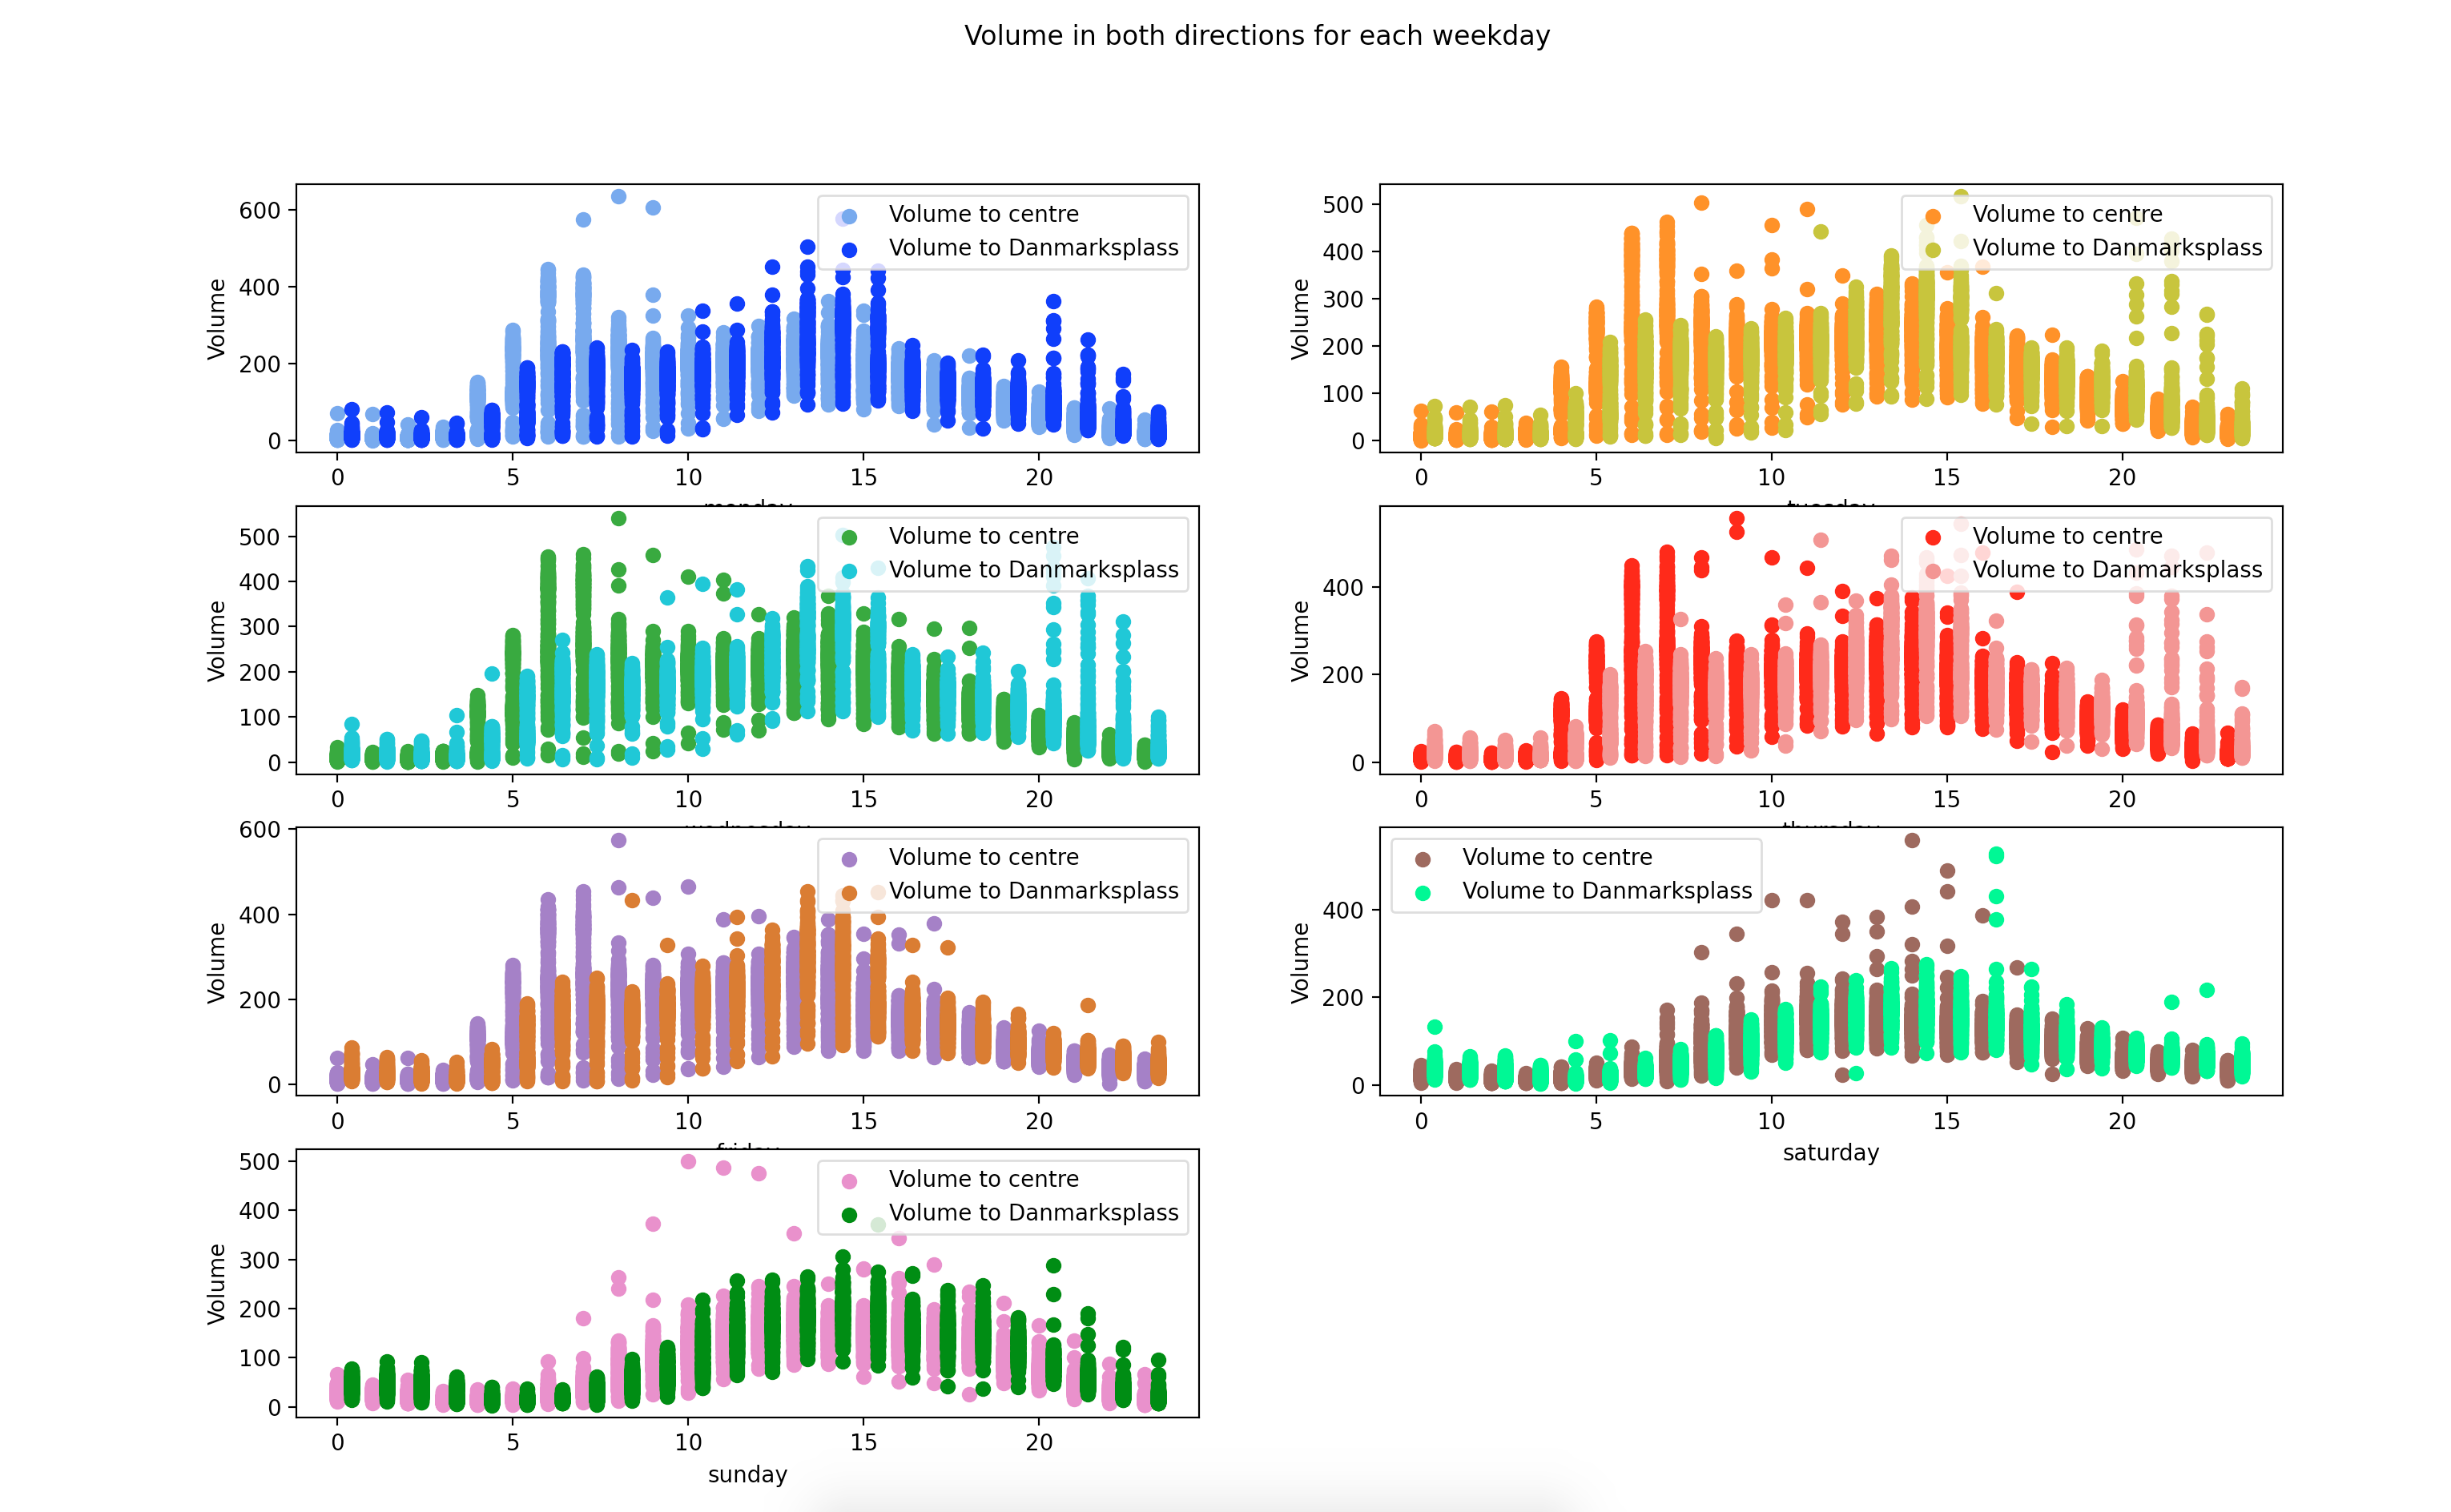
\includegraphics[scale = 0.29]{vis_days.png}
    \caption{Datapoints sorted by weekday}
    \label{fig::days}
\end{figure}

We do the same visualization for each month, to compare different seasons with each other.

\begin{figure}[h]
    \centering
    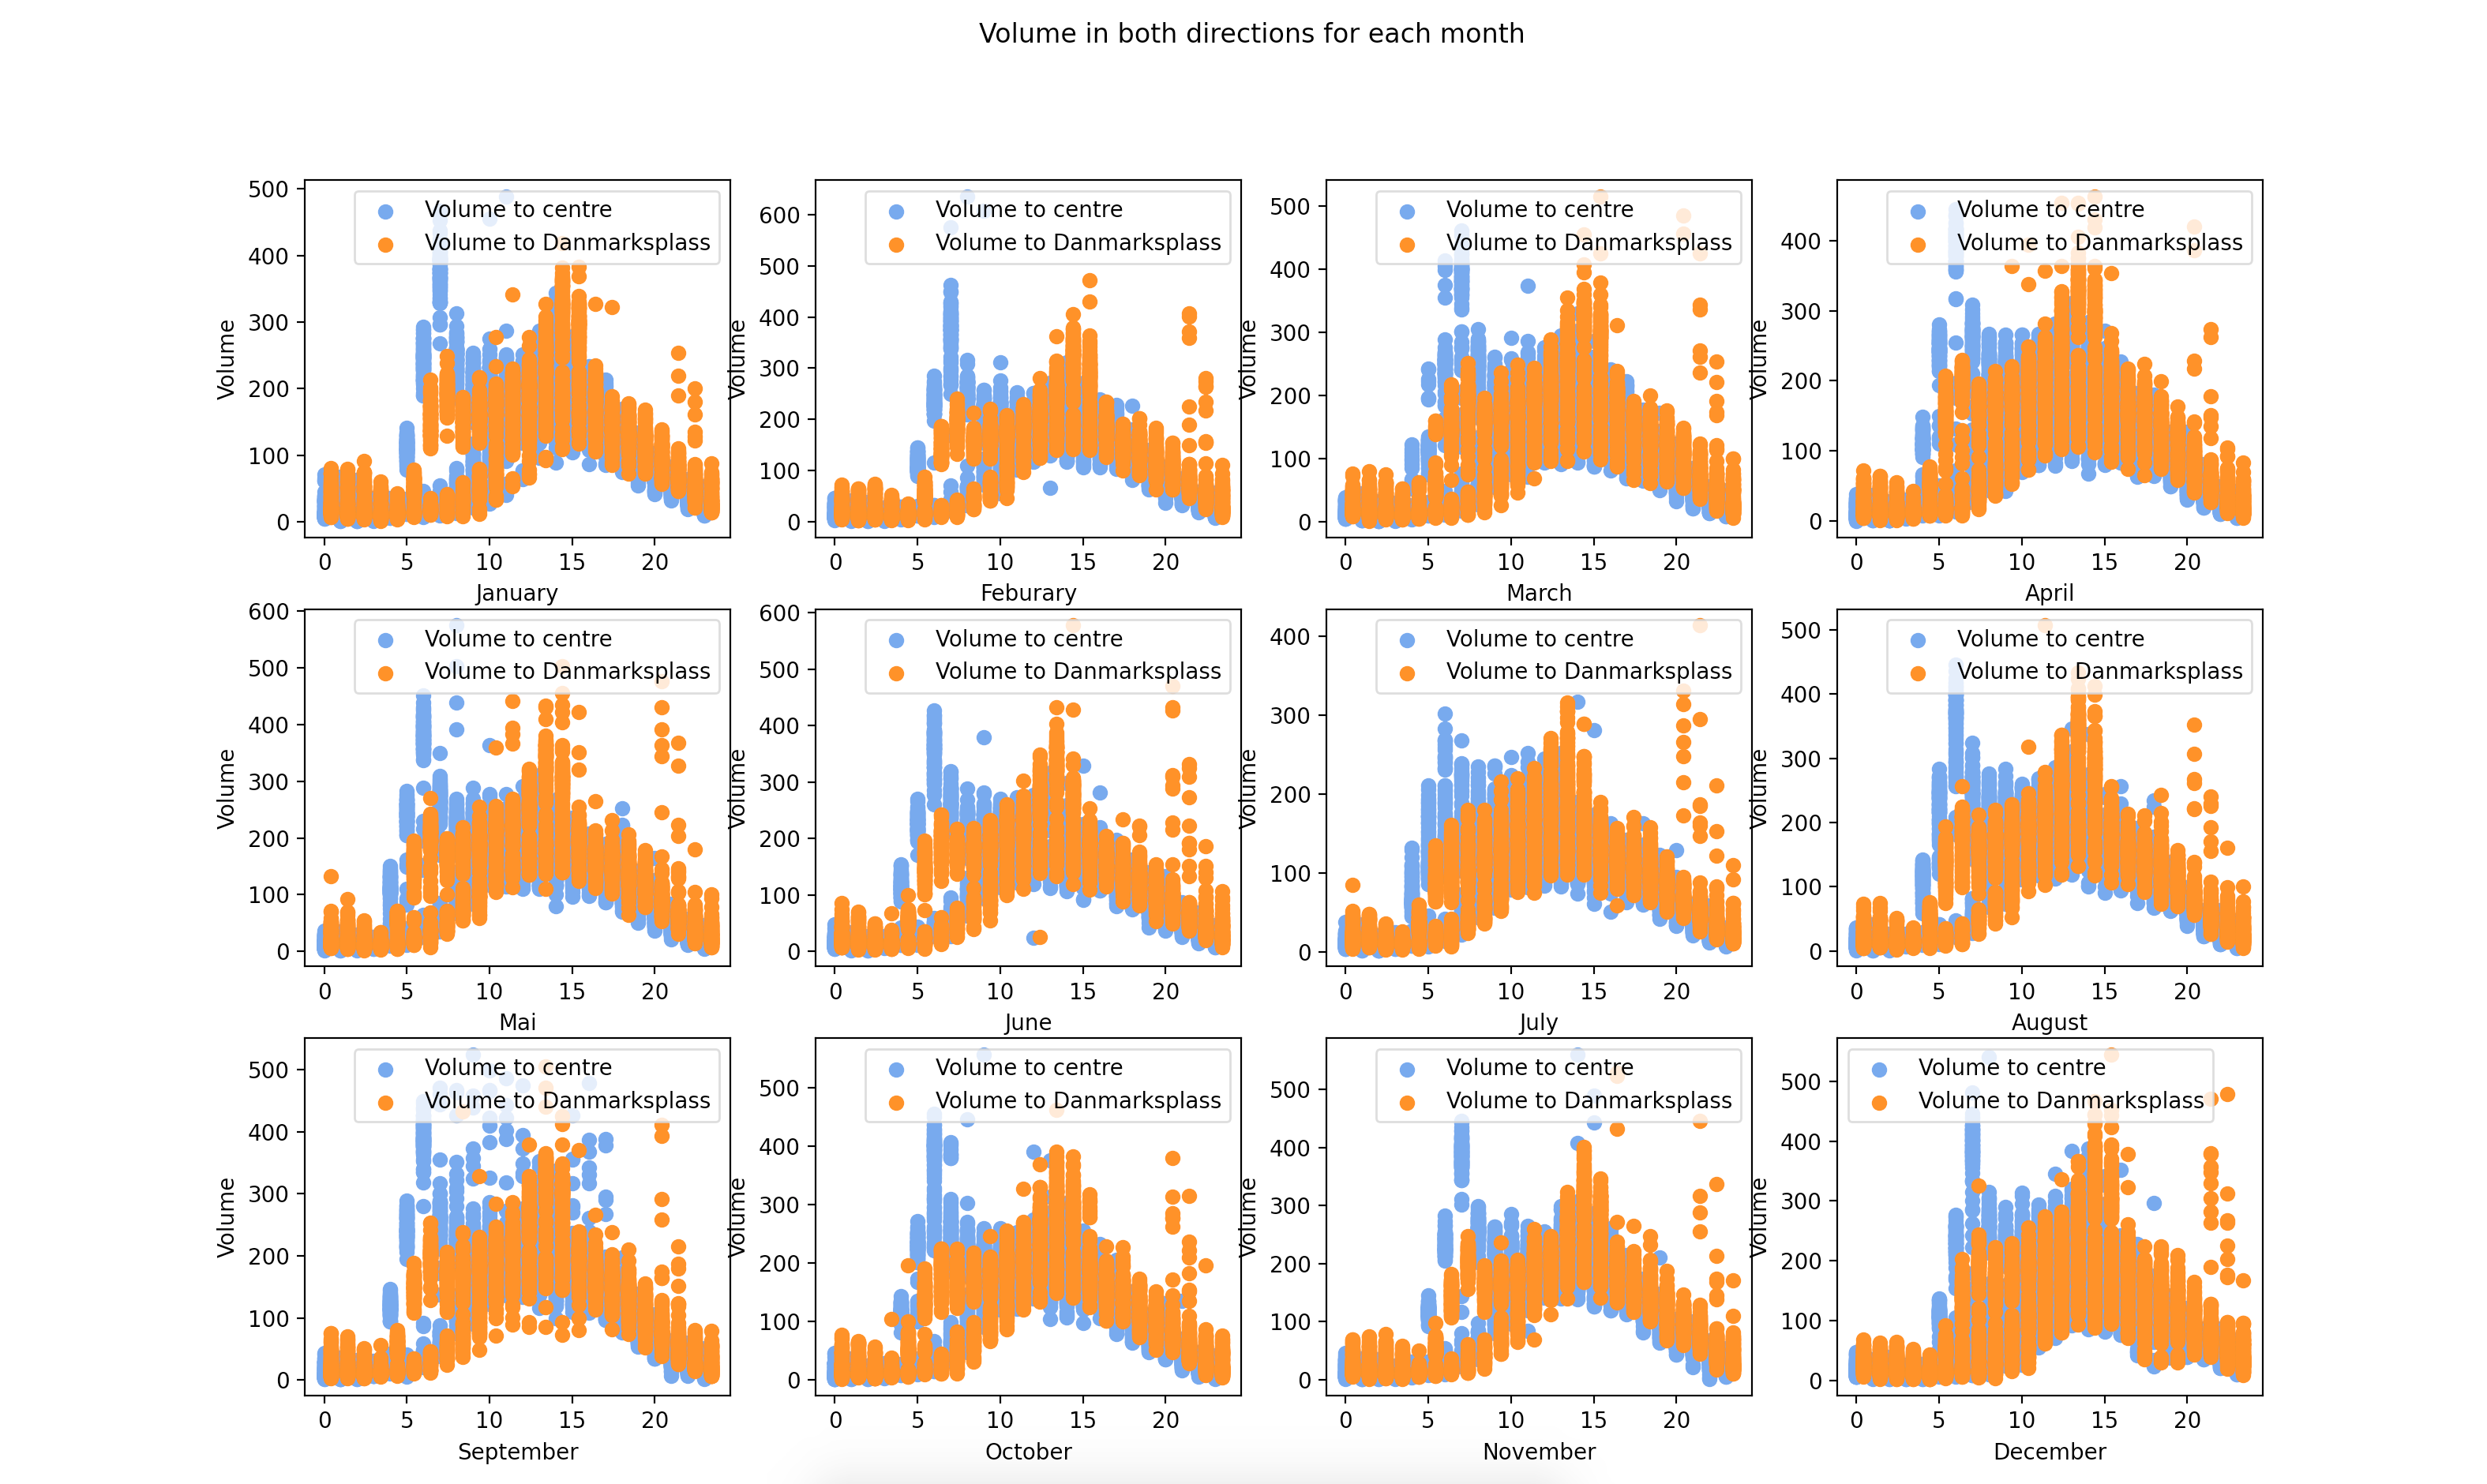
\includegraphics[scale = 0.28]{vis_months.png}
    \caption{Datapoints sorted by month}
    \label{fig::month}
\end{figure}

\subsection{Feature engineering}
Looking closer figure \ref{fig::days}, there are a few observations to make. 
The patterns differ indeed from weekdays to sundays, but saturdays have a pattern of their own as well.
There seems to be more traffic around the afternoon time (likeley the after work rush hour) out of the city centre 
and in the morning into the city centre. At night there is a lot less traffic overall.
The differences between the two directions are most visible during the rush hour times. 
The day could be seperated into daytime blocks to get simpler features, but we decide against that. 
Our reason for that is, that the overall pattern is divisible into blocks, but every hour still has a significant
difference to its neighbouring hours, so we decided to treat the hours of the day as continuous features.
Having a continuous feature for every single date at the same time is not very useful. As we can already see in this 
diagram, the biggest difference is between different weekdays. 
Instead of having the dates as features, we sort the datapoints according to their weekdays and make one-hot-encoding 
features out of it. Every date belongs to one of the three categories: weekday, saturday, sunday/holiday.
As holidays are similar to sundays cocnerning traffic (because there is no rush hour), we take the effort to sort out 
all the holidays as well and declare them as sundays.

To verify our feature choice as it is, we also look at the differences between each month (figure \ref{fig::month}).
We suspect a difference between the seasons, especially winter and summer as there may be less people driving with a car 
in the summer time and rather taking a bike. Looking at the diagram we can't spot significant differences, so we decide 
to not use the season of a given date as an additional feature.

\begin{lstlisting}[language=Python]
\end{lstlisting}


\end{document}